\documentclass[11pt,a4paper]{report}
\usepackage{anuthesis}
\usepackage{amssymb}
\usepackage{fancyhdr}
\usepackage{graphicx}
\usepackage{tikz}
\newcommand*\circled[1]{\tikz[baseline=(char.base)]{
            \node[shape=circle,draw,inner sep=2pt] (char) {#1};}}
  \renewcommand{\bottomfraction}{0.7}  

\begin{document}
\pagenumbering{roman}  % first use Roman numerals for page numbers

\begin{titlepage}
\title{\textbf{CSP and LP models of IQ Twist and Cube Puzzler - Go}\\[2cm]}
 \author{\textbf{Mingzhen Ao}\\[6cm]
 \textbf{A thesis submitted for the course}\\
 \textbf{COMP8755 Individual Computing Project} \\
 \textbf{Supervised by: Pascal Bercher and Florian Geisser}\\
 \textbf{The Australian National University}\\[1cm]}
 \date{\textbf{November, 2020}}
\maketitle
 \end{titlepage}
 
 \sloppy
 
\chapter*{Declaration}
\addcontentsline{toc}{chapter}{Declaration}

This thesis is an account of research undertaken between July 2020 and 
November 2020 at The College of Engineering and Computer Science, Faculty of Computing Science, The Australian National University, Canberra, Australia.

Except where acknowledged in the customary manner, the material 
presented in this thesis is, to the best of my knowledge, original and 
has not been submitted in whole or part for a degree in any 
university.

\vspace{20mm}  % vertical space

\hspace{80mm}\rule{40mm}{.15mm}\par   % horizontal space, line, start new line
\hspace{80mm} Mingzhen Ao\par
\hspace{80mm} November, 2020

% include statements effectively insert the contents of the named file.
% They are not necessary, but are useful for organising your work.
% They always start a  new page.

\chapter*{Acknowledgements}
\addcontentsline{toc}{chapter}{Acknowledgements}

I would like to thank my lucky stars, and the cat, for not eating me.
  % include the contents of the file thanks.tex

\chapter*{Abstract}
\addcontentsline{toc}{chapter}{Abstract}
\vspace{-1em}
The constraint satisfaction problems (CSPs) are created to model two puzzle games IQ Twist and Zig Zag Puzzler. Both of them have "start", "junior", "expert", "master" and "wizard" difficulties. With regard to CSPs for both games, the variables, domains, and constraints are mainly discussed. Meanwhile, in the process of discussing constraints, the 2D rotation matrix is introduced to clarify the pieces' configurations for the 2D game (IQ Twist), and the 3D rotation matrix is introduced to clarify the pieces' configurations for the 3D game (Zig Zag Puzzler). After that, these models are encoded by Minizinc which is a constraint modeling language. Through Minizinc IDE, the Minizinc is transferred to Flatzinc, a solver input language that is understood by a wide range of solvers. Therefore, nine solvers are used to execute these problems by different interfaces, which create the bridges between each solver and the Flatzinc file. For IQ Twist, the solvers' performances are not strongly related to the difficulties, while there is an obvious negative correlation between the performance and difficulties in Zig Zag Puzzler. Finally, there are three solvers Chuffed, OR-Tools and PicatSAT, which perform the 100 percent coverage. In other words,  they solve each problem in thirty minutes. More specifically, Chuffed achieve the optimal performance in most problems because it solves each problem in 20 seconds, while the other two need more time.
\\
\\
\\
\\\textbf{Keywords:} CSPs, IQ Twist, Zig Zag Puzzler, rotation matrix, Minizinc, Flatzinc, Chuffed, OR-Tools, PicatSAT.


  % include the file abstract.tex

\tableofcontents


\pagenumbering{arabic} % switch to Arabic numerals for page numbers
\setcounter{page}{1}  % set page number to 1

\chapter{Introduction}


  % include the file chapter1.tex

\chapter{IQ twist}
\section{CSP model}
\newcommand{\VUnits} {\ensuremath{V_{units}}}
\newcommand{\VPegs} {\ensuremath{V_{pegs}}}
\newcommand{\Constraints}[2] {\ensuremath{C_{v_{#1},v_{#2}}}}
\newcommand{\Cons}[5] {\ensuremath{C_{v_{#1},v_{#2},v_{#3},v_{#4},v_{#5}}}}
\newcommand{\Con}[4] {\ensuremath{C_{v_{#1},v_{#2},v_{#3},v_{#4}}}}
\newcommand{\Constraint}[1] {\ensuremath{C_{v_{#1}}}}
\newcommand{\Domain}[1] {\ensuremath{D(v_{#1})}}
\label{sec:CSP model}
In this part, I'd like to use CSP to model the IQ twist game. Above all, I'd like to define all the initial state for each piece:
\begin{center}

\includegraphics{yellow1.jpg} 
\\initial state of Yellow 1
\\
\includegraphics{yellow2.jpg}
\\initial state of Yellow 2
\\
\includegraphics{blue1.jpg}
\\initial state of Blue 1
\\
\includegraphics{blue2.jpg}
\\initial state of Blue 2
\\
\includegraphics{green1.jpg}
\\initial state of Green 1 
\\
\includegraphics{green2.jpg}
\\initial state of Green 2
\\
\includegraphics{red1.jpg}
\\initial state of Red 1 
\\
\includegraphics{red2.jpg}
\\initial state of Red 2 
\end{center}
For this method, there are some rules. Firstly, all the variables correspond to the initial states. Such as the Yellow 2, I use $V_{y21}$ to represent the left and bottom unit. For other variables, name them as $V_{y22}$, $V_{y23}$, $V_{y24}$ and $V_{y25}$ follow the order from left to right and bottom up.
\begin{center}
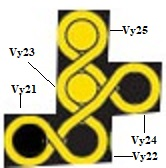
\includegraphics{example.jpg}
\\naming rules example for yellow 2
\end{center}
\subsection{Variables}

$\VUnits=\{ V_{y11},V_{y12},
V_{y13},V_{y21},V_{y22},V_{y23},V_{y24},V_{y25},\\V_{b11},V_{b12},V_{b13},V_{b14},
V_{b15},V_{b21},V_{b22},V_{b23},\\V_{b24},V_{g11},V_{g12},V_{g13},V_{g14},V_{g21},V_{g22},V_{g23},\\V_{r11},
V_{r12},V_{r13},V_{r14},V_{r21},V_{r22},V_{r23},V_{r24}\}$\\
\\$\VPegs = \{V_{py1}, V_{py2}, V_{pb1}, V_{pb2}, V_{pg1}, V_{pg2}, V_{pr}\}$\\
\\$V = \VUnits \cup \VPegs.$
\subsection{Domains}
$For \hspace{1ex} all \hspace{1ex} v \in \VUnits \hspace{1ex},\hspace{1ex} D(v)=\{(i,j) \in \mathbb{Z} \times \mathbb{Z}	\mid  0<i \leq 8 \hspace{1ex} , \hspace{1ex} 0<j \leq 4\}$\\
\\
$For \hspace{1ex} all \hspace{1ex} v \in \VPegs \hspace{1ex},\hspace{1ex} D(v)=\{(0,0)\} \hspace{1ex} \cup \hspace{1ex}\{(i,j) \in \mathbb{Z} \times \mathbb{Z}\mid  0<i \leq 8 \hspace{1ex} , \hspace{1ex} 0<j \leq 4\}$
\subsection{Constrains}
\circled{1} $For \hspace{1ex} each \hspace{1ex} pair\hspace{1ex} of \hspace{1ex}variables-V_{m} \hspace{1ex} and \hspace{1ex} V_{n}, V_{m} \in \VUnits, V_{n} \in \VUnits,$
\begin{center}
$\Constraints{m}{n}=\{((a,b),(c,d))\in \Domain{m} \times \Domain{n}\mid a \neq c   \hspace{1ex} or \hspace{1ex}  b \neq d\}$
\end{center}
\circled{2} 
$For \hspace{1ex} each \hspace{1ex} pair \hspace{1ex} of\hspace{1ex} variables-V_{m}\hspace{1ex} and \hspace{1ex}V_{n}, V_{m} \in \VPegs, V_{n} \in \VPegs,$
\begin{center}
$\Constraints{m}{n}=\{((0,0),(0,0))\}\cup \{((a,b),(c,d))\in \Domain{m}\times \Domain{n}\mid a \neq c   \hspace{1ex} or \hspace{1ex}  b \neq d\}$\\
\end{center}
\circled{3} piece Yellow1
\\$\Constraints{y11}{y12}=\{((a,b),(c,d))\in \Domain{y11}\times \Domain{y12}\mid c = a + 1\hspace{1ex} , \hspace{1ex}  d = b + 0 \}$ , 
\\$\Constraints{y11}{y13}=\{((a,b),(c,d))\in \Domain{y11}\times \Domain{y13}\mid c = a + 2\hspace{1ex} , \hspace{1ex}  d = b + 0 \}$ , 
\\$\cup$
\\$\Constraints{y11}{y12}=\{((a,b),(c,d))\in \Domain{y11}\times \Domain{y12}\mid c = a - 0\hspace{1ex} , \hspace{1ex}  d = b + 1 \}$ , 
\\$\Constraints{y11}{y13}=\{((a,b),(c,d))\in \Domain{y11}\times \Domain{y13}\mid c = a - 0\hspace{1ex} , \hspace{1ex}  d = b + 2 \}$ , 
\\$\cup$
\\$\Constraints{y11}{y12}=\{((a,b),(c,d))\in \Domain{y11}\times \Domain{y12}\mid c = a - 1\hspace{1ex} , \hspace{1ex}  d = b - 0 \}$ , 
\\$\Constraints{y11}{y13}=\{((a,b),(c,d))\in \Domain{y11}\times \Domain{y13}\mid c = a - 2\hspace{1ex} , \hspace{1ex}  d = b - 0 \}$ , 
\\$\cup$
\\$\Constraints{y11}{y12}=\{((a,b),(c,d))\in \Domain{y11}\times \Domain{y12}\mid c = a + 0\hspace{1ex} , \hspace{1ex}  d = b - 1 \}$ , 
\\$\Constraints{y11}{y13}=\{((a,b),(c,d))\in \Domain{y11}\times \Domain{y13}\mid c = a + 0\hspace{1ex} , \hspace{1ex}  d = b - 2 \}$ , 
\\$\cup$
\\$\Constraints{y11}{y12}=\{((a,b),(c,d))\in \Domain{y11}\times \Domain{y12}\mid c = a - 1\hspace{1ex} , \hspace{1ex}  d = b + 0 \}$ , 
\\$\Constraints{y11}{y13}=\{((a,b),(c,d))\in \Domain{y11}\times \Domain{y13}\mid c = a - 2\hspace{1ex} , \hspace{1ex}  d = b + 0 \}$ , 
\\$\cup$
\\$\Constraints{y11}{y12}=\{((a,b),(c,d))\in \Domain{y11}\times \Domain{y12}\mid c = a - 0\hspace{1ex} , \hspace{1ex}  d = b - 1 \}$ , 
\\$\Constraints{y11}{y13}=\{((a,b),(c,d))\in \Domain{y11}\times \Domain{y13}\mid c = a - 0\hspace{1ex} , \hspace{1ex}  d = b - 2 \}$ , 
\\$\cup$
\\$\Constraints{y11}{y12}=\{((a,b),(c,d))\in \Domain{y11}\times \Domain{y12}\mid c = a + 1\hspace{1ex} , \hspace{1ex}  d = b - 0 \}$ , 
\\$\Constraints{y11}{y13}=\{((a,b),(c,d))\in \Domain{y11}\times \Domain{y13}\mid c = a + 2\hspace{1ex} , \hspace{1ex}  d = b - 0 \}$ , 
\\$\cup$
\\$\Constraints{y11}{y12}=\{((a,b),(c,d))\in \Domain{y11}\times \Domain{y12}\mid c = a + 0\hspace{1ex} , \hspace{1ex}  d = b + 1 \}$ , 
\\$\Constraints{y11}{y13}=\{((a,b),(c,d))\in \Domain{y11}\times \Domain{y13}\mid c = a + 0\hspace{1ex} , \hspace{1ex}  d = b + 2 \}$ , 
\\\circled{4} piece Yellow2
\\$\Constraints{y21}{y22}=\{((a,b),(c,d))\in \Domain {y21} \times \Domain{y22} \mid c = a + 1\hspace{1ex} , \hspace{1ex}  d = b + 0 \}$ , 
\\$\Constraints{y21}{y23}=\{((a,b),(c,d))\in \Domain{y21} \times \Domain{y23}\mid c = a + 1\hspace{1ex} , \hspace{1ex}  d = b + 1 \}$ , 
\\$\Constraints{y21}{y24}=\{((a,b),(c,d))\in \Domain{y21} \times \Domain{y24}\mid c = a + 2\hspace{1ex} , \hspace{1ex}  d = b + 1 \}$ , 
\\$\Constraints{y21}{y25}=\{((a,b),(c,d))\in \Domain{y21} \times \Domain{y25}\mid c = a + 1\hspace{1ex} , \hspace{1ex}  d = b + 2 \}$ , 
\\$\cup$
\\$\Constraints{y21}{y22}=\{((a,b),(c,d))\in \Domain{y21} \times \Domain{y22}\mid c = a - 0\hspace{1ex} , \hspace{1ex}  d = b + 1 \}$ , 
\\$\Constraints{y21}{y23}=\{((a,b),(c,d))\in \Domain{y21} \times \Domain{y23}\mid c = a - 1\hspace{1ex} , \hspace{1ex}  d = b + 1 \}$ , 
\\$\Constraints{y21}{y24}=\{((a,b),(c,d))\in \Domain{y21} \times \Domain{y24}\mid c = a - 1\hspace{1ex} , \hspace{1ex}  d = b + 2 \}$ , 
\\$\Constraints{y21}{y25}=\{((a,b),(c,d))\in \Domain{y21} \times \Domain{y25}\mid c = a - 2\hspace{1ex} , \hspace{1ex}  d = b + 1 \}$ , 
\\$\cup$
\\$\Constraints{y21}{y22}=\{((a,b),(c,d))\in \Domain{y21} \times \Domain{y22}\mid c = a - 1\hspace{1ex} , \hspace{1ex}  d = b - 0 \}$ , 
\\$\Constraints{y21}{y23}=\{((a,b),(c,d))\in \Domain{y21} \times \Domain{y23}\mid c = a - 1\hspace{1ex} , \hspace{1ex}  d = b - 1 \}$ , 
\\$\Constraints{y21}{y24}=\{((a,b),(c,d))\in \Domain{y21} \times \Domain{y24}\mid c = a - 2\hspace{1ex} , \hspace{1ex}  d = b - 1 \}$ , 
\\$\Constraints{y21}{y25}=\{((a,b),(c,d))\in \Domain{y21} \times \Domain{y25}\mid c = a - 1\hspace{1ex} , \hspace{1ex}  d = b - 2 \}$ , 
\\$\cup$
\\$\Constraints{y21}{y22}=\{((a,b),(c,d))\in \Domain{y21} \times \Domain{y22}\mid c = a + 0\hspace{1ex} , \hspace{1ex}  d = b - 1 \}$ , 
\\$\Constraints{y21}{y23}=\{((a,b),(c,d))\in \Domain{y21} \times \Domain{y23}\mid c = a + 1\hspace{1ex} , \hspace{1ex}  d = b - 1 \}$ , 
\\$\Constraints{y21}{y24}=\{((a,b),(c,d))\in \Domain{y21} \times \Domain{y24}\mid c = a + 1\hspace{1ex} , \hspace{1ex}  d = b - 2 \}$ , 
\\$\Constraints{y21}{y25}=\{((a,b),(c,d))\in \Domain{y21} \times \Domain{y25}\mid c = a + 2\hspace{1ex} , \hspace{1ex}  d = b - 1 \}$ , 
\\$\cup$
\\$\Constraints{y21}{y22}=\{((a,b),(c,d))\in \Domain{y21} \times \Domain{y22}\mid c = a - 1\hspace{1ex} , \hspace{1ex}  d = b + 0 \}$ , 
\\$\Constraints{y21}{y23}=\{((a,b),(c,d))\in \Domain{y21} \times \Domain{y23}\mid c = a - 1\hspace{1ex} , \hspace{1ex}  d = b + 1 \}$ , 
\\$\Constraints{y21}{y24}=\{((a,b),(c,d))\in \Domain{y21} \times \Domain{y24}\mid c = a - 2\hspace{1ex} , \hspace{1ex}  d = b + 1 \}$ , 
\\$\Constraints{y21}{y25}=\{((a,b),(c,d))\in \Domain{y21} \times \Domain{y25}\mid c = a - 1\hspace{1ex} , \hspace{1ex}  d = b + 2 \}$ , 
\\$\cup$
\\$\Constraints{y21}{y22}=\{((a,b),(c,d))\in \Domain{y21} \times \Domain{y22}\mid c = a - 0\hspace{1ex} , \hspace{1ex}  d = b - 1 \}$ , 
\\$\Constraints{y21}{y23}=\{((a,b),(c,d))\in \Domain{y21} \times \Domain{y23}\mid c = a - 1\hspace{1ex} , \hspace{1ex}  d = b - 1 \}$ , 
\\$\Constraints{y21}{y24}=\{((a,b),(c,d))\in \Domain{y21} \times \Domain{y24}\mid c = a - 1\hspace{1ex} , \hspace{1ex}  d = b - 2 \}$ , 
\\$\Constraints{y21}{y25}=\{((a,b),(c,d))\in \Domain{y21} \times \Domain{y25}\mid c = a - 2\hspace{1ex} , \hspace{1ex}  d = b - 1 \}$ , 
\\$\cup$
\\$\Constraints{y21}{y22}=\{((a,b),(c,d))\in \Domain{y21} \times \Domain{y22}\mid c = a + 1\hspace{1ex} , \hspace{1ex}  d = b - 0 \}$ , 
\\$\Constraints{y21}{y23}=\{((a,b),(c,d))\in \Domain{y21} \times \Domain{y23}\mid c = a + 1\hspace{1ex} , \hspace{1ex}  d = b - 1 \}$ , 
\\$\Constraints{y21}{y24}=\{((a,b),(c,d))\in \Domain{y21} \times \Domain{y24}\mid c = a + 2\hspace{1ex} , \hspace{1ex}  d = b - 1 \}$ , 
\\$\Constraints{y21}{y25}=\{((a,b),(c,d))\in \Domain{y21} \times \Domain{y25}\mid c = a + 1\hspace{1ex} , \hspace{1ex}  d = b - 2 \}$ , 
\\$\cup$
\\$\Constraints{y21}{y22}=\{((a,b),(c,d))\in \Domain{y21} \times \Domain{y22}\mid c = a + 0\hspace{1ex} , \hspace{1ex}  d = b + 1 \}$ , 
\\$\Constraints{y21}{y23}=\{((a,b),(c,d))\in \Domain{y21} \times \Domain{y23}\mid c = a + 1\hspace{1ex} , \hspace{1ex}  d = b + 1 \}$ , 
\\$\Constraints{y21}{y24}=\{((a,b),(c,d))\in \Domain{y21} \times \Domain{y24}\mid c = a + 1\hspace{1ex} , \hspace{1ex}  d = b + 2 \}$ , 
\\$\Constraints{y21}{y25}=\{((a,b),(c,d))\in \Domain{y21} \times \Domain{y25}\mid c = a + 2\hspace{1ex} , \hspace{1ex}  d = b + 1 \}$ , 
\\\circled{5} piece Blue1 
\\$\Constraints{b11}{b12}=\{((a,b),(c,d))\in \Domain{b11} \times \Domain{b12}\mid c = a + 0\hspace{1ex} , \hspace{1ex}  d = b + 1 \}$ , 
\\$\Constraints{b11}{b13}=\{((a,b),(c,d))\in \Domain{b11} \times \Domain{b13}\mid c = a + 1\hspace{1ex} , \hspace{1ex}  d = b + 1 \}$ , 
\\$\Constraints{b11}{b14}=\{((a,b),(c,d))\in \Domain{b11} \times \Domain{y14}\mid c = a + 0\hspace{1ex} , \hspace{1ex}  d = b + 2 \}$ , 
\\$\Constraints{b11}{b15}=\{((a,b),(c,d))\in \Domain{b11} \times \Domain{b15}\mid c = a + 1\hspace{1ex} , \hspace{1ex}  d = b + 2 \}$ , 
\\$\cup$
\\$\Constraints{b11}{b12}=\{((a,b),(c,d))\in \Domain{b11} \times \Domain{b12}\mid c = a - 1\hspace{1ex} , \hspace{1ex}  d = b + 0 \}$ , 
\\$\Constraints{b11}{b13}=\{((a,b),(c,d))\in \Domain{b11} \times \Domain{b13}\mid c = a - 1\hspace{1ex} , \hspace{1ex}  d = b + 1 \}$ , 
\\$\Constraints{b11}{b14}=\{((a,b),(c,d))\in \Domain{b11} \times \Domain{y14}\mid c = a - 2\hspace{1ex} , \hspace{1ex}  d = b + 0 \}$ , 
\\$\Constraints{b11}{b15}=\{((a,b),(c,d))\in \Domain{b11} \times \Domain{b15}\mid c = a - 2\hspace{1ex} , \hspace{1ex}  d = b + 1 \}$ , 
\\$\cup$
\\$\Constraints{b11}{b12}=\{((a,b),(c,d))\in \Domain{b11} \times \Domain{b12}\mid c = a - 0\hspace{1ex} , \hspace{1ex}  d = b - 1 \}$ , 
\\$\Constraints{b11}{b13}=\{((a,b),(c,d))\in \Domain{b11} \times \Domain{b13}\mid c = a - 1\hspace{1ex} , \hspace{1ex}  d = b - 1 \}$ , 
\\$\Constraints{b11}{b14}=\{((a,b),(c,d))\in \Domain{b11} \times \Domain{y14}\mid c = a - 0\hspace{1ex} , \hspace{1ex}  d = b - 2 \}$ , 
\\$\Constraints{b11}{b15}=\{((a,b),(c,d))\in \Domain{b11} \times \Domain{b15}\mid c = a - 1\hspace{1ex} , \hspace{1ex}  d = b - 2 \}$ , 
\\$\cup$
\\$\Constraints{b11}{b12}=\{((a,b),(c,d))\in \Domain{b11} \times \Domain{b12}\mid c = a + 1\hspace{1ex} , \hspace{1ex}  d = b - 0 \}$ , 
\\$\Constraints{b11}{b13}=\{((a,b),(c,d))\in \Domain{b11} \times \Domain{b13}\mid c = a + 1\hspace{1ex} , \hspace{1ex}  d = b - 1 \}$ , 
\\$\Constraints{b11}{b14}=\{((a,b),(c,d))\in \Domain{b11} \times \Domain{y14}\mid c = a + 2\hspace{1ex} , \hspace{1ex}  d = b - 0 \}$ , 
\\$\Constraints{b11}{b15}=\{((a,b),(c,d))\in \Domain{b11} \times \Domain{b15}\mid c = a + 2\hspace{1ex} , \hspace{1ex}  d = b - 1 \}$ , 
\\$\cup$
\\$\Constraints{b11}{b12}=\{((a,b),(c,d))\in \Domain{b11} \times \Domain{b12}\mid c = a - 0\hspace{1ex} , \hspace{1ex}  d = b + 1 \}$ , 
\\$\Constraints{b11}{b13}=\{((a,b),(c,d))\in \Domain{b11} \times \Domain{b13}\mid c = a - 1\hspace{1ex} , \hspace{1ex}  d = b + 1 \}$ , 
\\$\Constraints{b11}{b14}=\{((a,b),(c,d))\in \Domain{b11} \times \Domain{y14}\mid c = a - 0\hspace{1ex} , \hspace{1ex}  d = b + 2 \}$ , 
\\$\Constraints{b11}{b15}=\{((a,b),(c,d))\in \Domain{b11} \times \Domain{b15}\mid c = a - 1\hspace{1ex} , \hspace{1ex}  d = b + 2 \}$ , 
\\$\cup$
\\$\Constraints{b11}{b12}=\{((a,b),(c,d))\in \Domain{b11} \times \Domain{b12}\mid c = a - 1\hspace{1ex} , \hspace{1ex}  d = b - 0 \}$ , 
\\$\Constraints{b11}{b13}=\{((a,b),(c,d))\in \Domain{b11} \times \Domain{b13}\mid c = a - 1\hspace{1ex} , \hspace{1ex}  d = b - 1 \}$ , 
\\$\Constraints{b11}{b14}=\{((a,b),(c,d))\in \Domain{b11} \times \Domain{y14}\mid c = a - 2\hspace{1ex} , \hspace{1ex}  d = b - 0 \}$ , 
\\$\Constraints{b11}{b15}=\{((a,b),(c,d))\in \Domain{b11} \times \Domain{b15}\mid c = a - 2\hspace{1ex} , \hspace{1ex}  d = b - 1 \}$ , 
\\$\cup$
\\$\Constraints{b11}{b12}=\{((a,b),(c,d))\in \Domain{b11} \times \Domain{b12}\mid c = a + 0\hspace{1ex} , \hspace{1ex}  d = b - 1 \}$ , 
\\$\Constraints{b11}{b13}=\{((a,b),(c,d))\in \Domain{b11} \times \Domain{b13}\mid c = a + 1\hspace{1ex} , \hspace{1ex}  d = b - 1 \}$ , 
\\$\Constraints{b11}{b14}=\{((a,b),(c,d))\in \Domain{b11} \times \Domain{y14}\mid c = a + 0\hspace{1ex} , \hspace{1ex}  d = b - 2 \}$ , 
\\$\Constraints{b11}{b15}=\{((a,b),(c,d))\in \Domain{b11} \times \Domain{b15}\mid c = a + 1\hspace{1ex} , \hspace{1ex}  d = b - 2 \}$ , 
\\$\cup$
\\$\Constraints{b11}{b12}=\{((a,b),(c,d))\in \Domain{b11} \times \Domain{b12}\mid c = a + 1\hspace{1ex} , \hspace{1ex}  d = b + 0 \}$ , 
\\$\Constraints{b11}{b13}=\{((a,b),(c,d))\in \Domain{b11} \times \Domain{b13}\mid c = a + 1\hspace{1ex} , \hspace{1ex}  d = b + 1 \}$ , 
\\$\Constraints{b11}{b14}=\{((a,b),(c,d))\in \Domain{b11} \times \Domain{y14}\mid c = a + 2\hspace{1ex} , \hspace{1ex}  d = b + 0 \}$ , 
\\$\Constraints{b11}{b15}=\{((a,b),(c,d))\in \Domain{b11} \times \Domain{b15}\mid c = a + 2\hspace{1ex} , \hspace{1ex}  d = b + 1 \}$ , 
\\\circled{6} piece Blue2 
\\$\Constraints{b21}{b22}=\{((a,b),(c,d))\in \Domain{b21} \times \Domain{b22}\mid c = a + 1\hspace{1ex} , \hspace{1ex}  d = b + 0 \}$ , 
\\$\Constraints{b21}{b23}=\{((a,b),(c,d))\in \Domain{b21} \times \Domain{b23}\mid c = a + 2\hspace{1ex} , \hspace{1ex}  d = b + 0 \}$ , 
\\$\Constraints{b21}{b24}=\{((a,b),(c,d))\in \Domain{b21} \times \Domain{b24}\mid c = a + 3\hspace{1ex} , \hspace{1ex}  d = b + 0 \}$ , 
\\$\cup$
\\$\Constraints{b21}{b22}=\{((a,b),(c,d))\in \Domain{b21} \times \Domain{b22}\mid c = a - 0\hspace{1ex} , \hspace{1ex}  d = b + 1 \}$ , 
\\$\Constraints{b21}{b23}=\{((a,b),(c,d))\in \Domain{b21} \times \Domain{b23}\mid c = a - 0\hspace{1ex} , \hspace{1ex}  d = b + 2 \}$ , 
\\$\Constraints{b21}{b24}=\{((a,b),(c,d))\in \Domain{b21} \times \Domain{b24}\mid c = a - 0\hspace{1ex} , \hspace{1ex}  d = b + 3 \}$ , 
\\$\cup$
\\$\Constraints{b21}{b22}=\{((a,b),(c,d))\in \Domain{b21} \times \Domain{b22}\mid c = a - 1\hspace{1ex} , \hspace{1ex}  d = b - 0 \}$ , 
\\$\Constraints{b21}{b23}=\{((a,b),(c,d))\in \Domain{b21} \times \Domain{b23}\mid c = a - 2\hspace{1ex} , \hspace{1ex}  d = b - 0 \}$ , 
\\$\Constraints{b21}{b24}=\{((a,b),(c,d))\in \Domain{b21} \times \Domain{b24}\mid c = a - 3\hspace{1ex} , \hspace{1ex}  d = b - 0 \}$ , 
\\$\cup$
\\$\Constraints{b21}{b22}=\{((a,b),(c,d))\in \Domain{b21} \times \Domain{b22}\mid c = a + 0\hspace{1ex} , \hspace{1ex}  d = b - 1 \}$ , 
\\$\Constraints{b21}{b23}=\{((a,b),(c,d))\in \Domain{b21} \times \Domain{b23}\mid c = a + 0\hspace{1ex} , \hspace{1ex}  d = b - 2 \}$ , 
\\$\Constraints{b21}{b24}=\{((a,b),(c,d))\in \Domain{b21} \times \Domain{b24}\mid c = a + 0\hspace{1ex} , \hspace{1ex}  d = b - 3 \}$ , 
\\$\cup$
\\$\Constraints{b21}{b22}=\{((a,b),(c,d))\in \Domain{b21} \times \Domain{b22}\mid c = a - 1\hspace{1ex} , \hspace{1ex}  d = b + 0 \}$ , 
\\$\Constraints{b21}{b23}=\{((a,b),(c,d))\in \Domain{b21} \times \Domain{b23}\mid c = a - 2\hspace{1ex} , \hspace{1ex}  d = b + 0 \}$ , 
\\$\Constraints{b21}{b24}=\{((a,b),(c,d))\in \Domain{b21} \times \Domain{b24}\mid c = a - 3\hspace{1ex} , \hspace{1ex}  d = b + 0 \}$ , 
\\$\cup$
\\$\Constraints{b21}{b22}=\{((a,b),(c,d))\in \Domain{b21} \times \Domain{b22}\mid c = a - 0\hspace{1ex} , \hspace{1ex}  d = b - 1 \}$ , 
\\$\Constraints{b21}{b23}=\{((a,b),(c,d))\in \Domain{b21} \times \Domain{b23}\mid c = a - 0\hspace{1ex} , \hspace{1ex}  d = b - 2 \}$ , 
\\$\Constraints{b21}{b24}=\{((a,b),(c,d))\in \Domain{b21} \times \Domain{b24}\mid c = a - 0\hspace{1ex} , \hspace{1ex}  d = b - 3 \}$ , 
\\$\cup$
\\$\Constraints{b21}{b22}=\{((a,b),(c,d))\in \Domain{b21} \times \Domain{b22}\mid c = a + 1\hspace{1ex} , \hspace{1ex}  d = b - 0 \}$ , 
\\$\Constraints{b21}{b23}=\{((a,b),(c,d))\in \Domain{b21} \times \Domain{b23}\mid c = a + 2\hspace{1ex} , \hspace{1ex}  d = b - 0 \}$ , 
\\$\Constraints{b21}{b24}=\{((a,b),(c,d))\in \Domain{b21} \times \Domain{b24}\mid c = a + 3\hspace{1ex} , \hspace{1ex}  d = b - 0 \}$ , 
\\$\cup$
\\$\Constraints{b21}{b22}=\{((a,b),(c,d))\in \Domain{b21} \times \Domain{b22}\mid c = a + 0\hspace{1ex} , \hspace{1ex}  d = b + 1 \}$ , 
\\$\Constraints{b21}{b23}=\{((a,b),(c,d))\in \Domain{b21} \times \Domain{b23}\mid c = a + 0\hspace{1ex} , \hspace{1ex}  d = b + 2 \}$ , 
\\$\Constraints{b21}{b24}=\{((a,b),(c,d))\in \Domain{b21} \times \Domain{b24}\mid c = a + 0\hspace{1ex} , \hspace{1ex}  d = b + 3 \}$ , 
\\\circled{7} piece Green1 
\\$\Constraints{g11}{g12}=\{((a,b),(c,d))\in \Domain{g11} \times \Domain{g12}\mid c = a + 1\hspace{1ex} , \hspace{1ex}  d = b + 0 \}$ , 
\\$\Constraints{g11}{g13}=\{((a,b),(c,d))\in \Domain{g11} \times \Domain{g13}\mid c = a + 2\hspace{1ex} , \hspace{1ex}  d = b + 0 \}$ , 
\\$\Constraints{g11}{g14}=\{((a,b),(c,d))\in \Domain{g11} \times \Domain{g14}\mid c = a + 1\hspace{1ex} , \hspace{1ex}  d = b + 1 \}$ , 
\\$\cup$
\\$\Constraints{g11}{g12}=\{((a,b),(c,d))\in \Domain{g11} \times \Domain{g12}\mid c = a - 0\hspace{1ex} , \hspace{1ex}  d = b + 1 \}$ , 
\\$\Constraints{g11}{g13}=\{((a,b),(c,d))\in \Domain{g11} \times \Domain{g13}\mid c = a - 0\hspace{1ex} , \hspace{1ex}  d = b + 2 \}$ , 
\\$\Constraints{g11}{g14}=\{((a,b),(c,d))\in \Domain{g11} \times \Domain{g14}\mid c = a - 1\hspace{1ex} , \hspace{1ex}  d = b + 1 \}$ , 
\\$\cup$
\\$\Constraints{g11}{g12}=\{((a,b),(c,d))\in \Domain{g11} \times \Domain{g12}\mid c = a - 1\hspace{1ex} , \hspace{1ex}  d = b - 0 \}$ , 
\\$\Constraints{g11}{g13}=\{((a,b),(c,d))\in \Domain{g11} \times \Domain{g13}\mid c = a - 2\hspace{1ex} , \hspace{1ex}  d = b - 0 \}$ , 
\\$\Constraints{g11}{g14}=\{((a,b),(c,d))\in \Domain{g11} \times \Domain{g14}\mid c = a - 1\hspace{1ex} , \hspace{1ex}  d = b - 1 \}$ , 
\\$\cup$
\\$\Constraints{g11}{g12}=\{((a,b),(c,d))\in \Domain{g11} \times \Domain{g12}\mid c = a + 0\hspace{1ex} , \hspace{1ex}  d = b - 1 \}$ , 
\\$\Constraints{g11}{g13}=\{((a,b),(c,d))\in \Domain{g11} \times \Domain{g13}\mid c = a + 0\hspace{1ex} , \hspace{1ex}  d = b - 2 \}$ , 
\\$\Constraints{g11}{g14}=\{((a,b),(c,d))\in \Domain{g11} \times \Domain{g14}\mid c = a + 1\hspace{1ex} , \hspace{1ex}  d = b - 1 \}$ , 
\\$\cup$
\\$\Constraints{g11}{g12}=\{((a,b),(c,d))\in \Domain{g11} \times \Domain{g12}\mid c = a - 1\hspace{1ex} , \hspace{1ex}  d = b + 0 \}$ , 
\\$\Constraints{g11}{g13}=\{((a,b),(c,d))\in \Domain{g11} \times \Domain{g13}\mid c = a - 2\hspace{1ex} , \hspace{1ex}  d = b + 0 \}$ , 
\\$\Constraints{g11}{g14}=\{((a,b),(c,d))\in \Domain{g11} \times \Domain{g14}\mid c = a - 1\hspace{1ex} , \hspace{1ex}  d = b + 1 \}$ , 
\\$\cup$
\\$\Constraints{g11}{g12}=\{((a,b),(c,d))\in \Domain{g11} \times \Domain{g12}\mid c = a - 0\hspace{1ex} , \hspace{1ex}  d = b - 1 \}$ , 
\\$\Constraints{g11}{g13}=\{((a,b),(c,d))\in \Domain{g11} \times \Domain{g13}\mid c = a - 0\hspace{1ex} , \hspace{1ex}  d = b - 2 \}$ , 
\\$\Constraints{g11}{g14}=\{((a,b),(c,d))\in \Domain{g11} \times \Domain{g14}\mid c = a - 1\hspace{1ex} , \hspace{1ex}  d = b - 1 \}$ , 
\\$\cup$
\\$\Constraints{g11}{g12}=\{((a,b),(c,d))\in \Domain{g11} \times \Domain{g12}\mid c = a + 1\hspace{1ex} , \hspace{1ex}  d = b - 0 \}$ , 
\\$\Constraints{g11}{g13}=\{((a,b),(c,d))\in \Domain{g11} \times \Domain{g13}\mid c = a + 2\hspace{1ex} , \hspace{1ex}  d = b - 0 \}$ , 
\\$\Constraints{g11}{g14}=\{((a,b),(c,d))\in \Domain{g11} \times \Domain{g14}\mid c = a + 1\hspace{1ex} , \hspace{1ex}  d = b - 1 \}$ , 
\\$\cup$
\\$\Constraints{g11}{g12}=\{((a,b),(c,d))\in \Domain{g11} \times \Domain{g12}\mid c = a + 0\hspace{1ex} , \hspace{1ex}  d = b + 1 \}$ , 
\\$\Constraints{g11}{g13}=\{((a,b),(c,d))\in \Domain{g11} \times \Domain{g13}\mid c = a + 0\hspace{1ex} , \hspace{1ex}  d = b + 2 \}$ , 
\\$\Constraints{g11}{g14}=\{((a,b),(c,d))\in \Domain{g11} \times \Domain{g14}\mid c = a + 1\hspace{1ex} , \hspace{1ex}  d = b + 1 \}$ , 
\\\circled{8} piece Green2 
\\$\Constraints{g21}{g22}=\{((a,b),(c,d))\in\Domain{g21} \times \Domain{g22}\mid c = a + 1\hspace{1ex} , \hspace{1ex}  d = b + 0 \}$ , 
\\$\Constraints{g21}{g23}=\{((a,b),(c,d))\in \Domain{g21} \times \Domain{g23}\mid c = a + 1\hspace{1ex} , \hspace{1ex}  d = b + 1 \}$ , 
\\$\cup$
\\$\Constraints{g21}{g22}=\{((a,b),(c,d))\in\Domain{g21} \times \Domain{g22}\mid c = a - 0\hspace{1ex} , \hspace{1ex}  d = b + 1 \}$ , 
\\$\Constraints{g21}{g23}=\{((a,b),(c,d))\in \Domain{g21} \times \Domain{g23}\mid c = a - 1\hspace{1ex} , \hspace{1ex}  d = b + 1 \}$ , 
\\$\cup$
\\$\Constraints{g21}{g22}=\{((a,b),(c,d))\in\Domain{g21} \times \Domain{g22}\mid c = a - 1\hspace{1ex} , \hspace{1ex}  d = b - 0 \}$ , 
\\$\Constraints{g21}{g23}=\{((a,b),(c,d))\in \Domain{g21} \times \Domain{g23}\mid c = a - 1\hspace{1ex} , \hspace{1ex}  d = b - 1 \}$ , 
\\$\cup$
\\$\Constraints{g21}{g22}=\{((a,b),(c,d))\in\Domain{g21} \times \Domain{g22}\mid c = a + 0\hspace{1ex} , \hspace{1ex}  d = b - 1 \}$ , 
\\$\Constraints{g21}{g23}=\{((a,b),(c,d))\in \Domain{g21} \times \Domain{g23}\mid c = a + 1\hspace{1ex} , \hspace{1ex}  d = b - 1 \}$ , 
\\$\cup$
\\$\Constraints{g21}{g22}=\{((a,b),(c,d))\in\Domain{g21} \times \Domain{g22}\mid c = a - 1\hspace{1ex} , \hspace{1ex}  d = b + 0 \}$ , 
\\$\Constraints{g21}{g23}=\{((a,b),(c,d))\in \Domain{g21} \times \Domain{g23}\mid c = a - 1\hspace{1ex} , \hspace{1ex}  d = b + 1 \}$ , 
\\$\cup$
\\$\Constraints{g21}{g22}=\{((a,b),(c,d))\in\Domain{g21} \times \Domain{g22}\mid c = a - 0\hspace{1ex} , \hspace{1ex}  d = b - 1 \}$ , 
\\$\Constraints{g21}{g23}=\{((a,b),(c,d))\in \Domain{g21} \times \Domain{g23}\mid c = a - 1\hspace{1ex} , \hspace{1ex}  d = b - 1 \}$ , 
\\$\cup$
\\$\Constraints{g21}{g22}=\{((a,b),(c,d))\in\Domain{g21} \times \Domain{g22}\mid c = a + 1\hspace{1ex} , \hspace{1ex}  d = b - 0 \}$ , 
\\$\Constraints{g21}{g23}=\{((a,b),(c,d))\in \Domain{g21} \times \Domain{g23}\mid c = a + 1\hspace{1ex} , \hspace{1ex}  d = b - 1 \}$ , 
\\$\cup$
\\$\Constraints{g21}{g22}=\{((a,b),(c,d))\in\Domain{g21} \times \Domain{g22}\mid c = a + 0\hspace{1ex} , \hspace{1ex}  d = b + 1 \}$ , 
\\$\Constraints{g21}{g23}=\{((a,b),(c,d))\in \Domain{g21} \times \Domain{g23}\mid c = a + 1\hspace{1ex} , \hspace{1ex}  d = b + 1 \}$ , 
\\\circled{9} piece Red1 
\\$\Constraints{r11}{r12}=\{((a,b),(c,d))\in \Domain{r11} \times \Domain{r12}\mid c = a + 1\hspace{1ex} , \hspace{1ex}  d = b + 0 \}$ , 
\\$\Constraints{r11}{r13}=\{((a,b),(c,d))\in \Domain{r11} \times \Domain{r13}\mid c = a + 1\hspace{1ex} , \hspace{1ex}  d = b + 1 \}$ , 
\\$\Constraints{r11}{r14}=\{((a,b),(c,d))\in \Domain{r11} \times \Domain{r14}\mid c = a + 2\hspace{1ex} , \hspace{1ex}  d = b + 1 \}$ , 
\\$\cup$
\\$\Constraints{r11}{r12}=\{((a,b),(c,d))\in \Domain{r11} \times \Domain{r12}\mid c = a - 0\hspace{1ex} , \hspace{1ex}  d = b + 1 \}$ , 
\\$\Constraints{r11}{r13}=\{((a,b),(c,d))\in \Domain{r11} \times \Domain{r13}\mid c = a - 1\hspace{1ex} , \hspace{1ex}  d = b + 1 \}$ , 
\\$\Constraints{r11}{r14}=\{((a,b),(c,d))\in \Domain{r11} \times \Domain{r14}\mid c = a - 1\hspace{1ex} , \hspace{1ex}  d = b + 2 \}$ , 
\\$\cup$
\\$\Constraints{r11}{r12}=\{((a,b),(c,d))\in \Domain{r11} \times \Domain{r12}\mid c = a - 1\hspace{1ex} , \hspace{1ex}  d = b - 0 \}$ , 
\\$\Constraints{r11}{r13}=\{((a,b),(c,d))\in \Domain{r11} \times \Domain{r13}\mid c = a - 1\hspace{1ex} , \hspace{1ex}  d = b - 1 \}$ , 
\\$\Constraints{r11}{r14}=\{((a,b),(c,d))\in \Domain{r11} \times \Domain{r14}\mid c = a - 2\hspace{1ex} , \hspace{1ex}  d = b - 1 \}$ , 
\\$\cup$
\\$\Constraints{r11}{r12}=\{((a,b),(c,d))\in \Domain{r11} \times \Domain{r12}\mid c = a + 0\hspace{1ex} , \hspace{1ex}  d = b - 1 \}$ , 
\\$\Constraints{r11}{r13}=\{((a,b),(c,d))\in \Domain{r11} \times \Domain{r13}\mid c = a + 1\hspace{1ex} , \hspace{1ex}  d = b - 1 \}$ , 
\\$\Constraints{r11}{r14}=\{((a,b),(c,d))\in \Domain{r11} \times \Domain{r14}\mid c = a + 1\hspace{1ex} , \hspace{1ex}  d = b - 2 \}$ , 
\\$\cup$
\\$\Constraints{r11}{r12}=\{((a,b),(c,d))\in \Domain{r11} \times \Domain{r12}\mid c = a - 1\hspace{1ex} , \hspace{1ex}  d = b + 0 \}$ , 
\\$\Constraints{r11}{r13}=\{((a,b),(c,d))\in \Domain{r11} \times \Domain{r13}\mid c = a - 1\hspace{1ex} , \hspace{1ex}  d = b + 1 \}$ , 
\\$\Constraints{r11}{r14}=\{((a,b),(c,d))\in \Domain{r11} \times \Domain{r14}\mid c = a - 2\hspace{1ex} , \hspace{1ex}  d = b + 1 \}$ , 
\\$\cup$
\\$\Constraints{r11}{r12}=\{((a,b),(c,d))\in \Domain{r11} \times \Domain{r12}\mid c = a - 0\hspace{1ex} , \hspace{1ex}  d = b - 1 \}$ , 
\\$\Constraints{r11}{r13}=\{((a,b),(c,d))\in \Domain{r11} \times \Domain{r13}\mid c = a - 1\hspace{1ex} , \hspace{1ex}  d = b - 1 \}$ , 
\\$\Constraints{r11}{r14}=\{((a,b),(c,d))\in \Domain{r11} \times \Domain{r14}\mid c = a - 1\hspace{1ex} , \hspace{1ex}  d = b - 2 \}$ , 
\\$\cup$
\\$\Constraints{r11}{r12}=\{((a,b),(c,d))\in \Domain{r11} \times \Domain{r12}\mid c = a + 1\hspace{1ex} , \hspace{1ex}  d = b - 0 \}$ , 
\\$\Constraints{r11}{r13}=\{((a,b),(c,d))\in \Domain{r11} \times \Domain{r13}\mid c = a + 1\hspace{1ex} , \hspace{1ex}  d = b - 1 \}$ , 
\\$\Constraints{r11}{r14}=\{((a,b),(c,d))\in \Domain{r11} \times \Domain{r14}\mid c = a + 2\hspace{1ex} , \hspace{1ex}  d = b - 1 \}$ , 
\\$\cup$
\\$\Constraints{r11}{r12}=\{((a,b),(c,d))\in \Domain{r11} \times \Domain{r12}\mid c = a + 0\hspace{1ex} , \hspace{1ex}  d = b + 1 \}$ , 
\\$\Constraints{r11}{r13}=\{((a,b),(c,d))\in \Domain{r11} \times \Domain{r13}\mid c = a + 1\hspace{1ex} , \hspace{1ex}  d = b + 1 \}$ , 
\\$\Constraints{r11}{r14}=\{((a,b),(c,d))\in \Domain{r11} \times \Domain{r14}\mid c = a + 1\hspace{1ex} , \hspace{1ex}  d = b + 2 \}$ , 
\\\circled{10} piece Red2 
\\$\Constraints{r21}{r22}=\{((a,b),(c,d))\in \Domain{r21} \times \Domain{r22}\mid c = a + 1\hspace{1ex} , \hspace{1ex}  d = b + 0 \}$ , 
\\$\Constraints{r21}{r23}=\{((a,b),(c,d))\in \Domain{r21} \times \Domain{r23}\mid c = a + 2\hspace{1ex} , \hspace{1ex}  d = b + 0 \}$ , 
\\$\Constraints{r21}{r24}=\{((a,b),(c,d))\in \Domain{r21} \times \Domain{r24}\mid c = a + 0\hspace{1ex} , \hspace{1ex}  d = b + 1 \}$ , 
\\$\cup$
\\$\Constraints{r21}{r22}=\{((a,b),(c,d))\in \Domain{r21} \times \Domain{r22}\mid c = a - 0\hspace{1ex} , \hspace{1ex}  d = b + 1 \}$ , 
\\$\Constraints{r21}{r23}=\{((a,b),(c,d))\in \Domain{r21} \times \Domain{r23}\mid c = a - 0\hspace{1ex} , \hspace{1ex}  d = b + 2 \}$ , 
\\$\Constraints{r21}{r24}=\{((a,b),(c,d))\in \Domain{r21} \times \Domain{r24}\mid c = a - 1\hspace{1ex} , \hspace{1ex}  d = b + 0 \}$ , 
\\$\cup$
\\$\Constraints{r21}{r22}=\{((a,b),(c,d))\in \Domain{r21} \times \Domain{r22}\mid c = a - 1\hspace{1ex} , \hspace{1ex}  d = b - 0 \}$ , 
\\$\Constraints{r21}{r23}=\{((a,b),(c,d))\in \Domain{r21} \times \Domain{r23}\mid c = a - 2\hspace{1ex} , \hspace{1ex}  d = b - 0 \}$ , 
\\$\Constraints{r21}{r24}=\{((a,b),(c,d))\in \Domain{r21} \times \Domain{r24}\mid c = a - 0\hspace{1ex} , \hspace{1ex}  d = b - 1 \}$ , 
\\$\cup$
\\$\Constraints{r21}{r22}=\{((a,b),(c,d))\in \Domain{r21} \times \Domain{r22}\mid c = a + 0\hspace{1ex} , \hspace{1ex}  d = b - 1 \}$ , 
\\$\Constraints{r21}{r23}=\{((a,b),(c,d))\in \Domain{r21} \times \Domain{r23}\mid c = a + 0\hspace{1ex} , \hspace{1ex}  d = b - 2 \}$ , 
\\$\Constraints{r21}{r24}=\{((a,b),(c,d))\in \Domain{r21} \times \Domain{r24}\mid c = a + 1\hspace{1ex} , \hspace{1ex}  d = b - 0 \}$ , 
\\$\cup$
\\$\Constraints{r21}{r22}=\{((a,b),(c,d))\in \Domain{r21} \times \Domain{r22}\mid c = a - 1\hspace{1ex} , \hspace{1ex}  d = b + 0 \}$ , 
\\$\Constraints{r21}{r23}=\{((a,b),(c,d))\in \Domain{r21} \times \Domain{r23}\mid c = a - 2\hspace{1ex} , \hspace{1ex}  d = b + 0 \}$ , 
\\$\Constraints{r21}{r24}=\{((a,b),(c,d))\in \Domain{r21} \times \Domain{r24}\mid c = a - 0\hspace{1ex} , \hspace{1ex}  d = b + 1 \}$ , 
\\$\cup$
\\$\Constraints{r21}{r22}=\{((a,b),(c,d))\in \Domain{r21} \times \Domain{r22}\mid c = a - 0\hspace{1ex} , \hspace{1ex}  d = b - 1 \}$ , 
\\$\Constraints{r21}{r23}=\{((a,b),(c,d))\in \Domain{r21} \times \Domain{r23}\mid c = a - 0\hspace{1ex} , \hspace{1ex}  d = b - 2 \}$ , 
\\$\Constraints{r21}{r24}=\{((a,b),(c,d))\in \Domain{r21} \times \Domain{r24}\mid c = a - 1\hspace{1ex} , \hspace{1ex}  d = b - 0 \}$ , 
\\$\cup$
\\$\Constraints{r21}{r22}=\{((a,b),(c,d))\in \Domain{r21} \times \Domain{r22}\mid c = a + 1\hspace{1ex} , \hspace{1ex}  d = b - 0 \}$ , 
\\$\Constraints{r21}{r23}=\{((a,b),(c,d))\in \Domain{r21} \times \Domain{r23}\mid c = a + 2\hspace{1ex} , \hspace{1ex}  d = b - 0 \}$ , 
\\$\Constraints{r21}{r24}=\{((a,b),(c,d))\in \Domain{r21} \times \Domain{r24}\mid c = a + 0\hspace{1ex} , \hspace{1ex}  d = b - 1 \}$ , 
\\$\cup$
\\$\Constraints{r21}{r22}=\{((a,b),(c,d))\in \Domain{r21} \times \Domain{r22}\mid c = a + 0\hspace{1ex} , \hspace{1ex}  d = b + 1 \}$ , 
\\$\Constraints{r21}{r23}=\{((a,b),(c,d))\in \Domain{r21} \times \Domain{r23}\mid c = a + 0\hspace{1ex} , \hspace{1ex}  d = b + 2 \}$ , 
\\$\Constraints{r21}{r24}=\{((a,b),(c,d))\in \Domain{r21} \times \Domain{r24}\mid c = a + 1\hspace{1ex} , \hspace{1ex}  d = b + 0 \}$ , 
\\\circled{11} Yellow peg1 
\\$\Cons{py1}{y11}{y21}{y22}{y24}= \{((a,b),(c,d))\in \Domain{py1} \times \Domain{y11}\mid c = a \hspace{1ex} , \hspace{1ex}  d = b\} \hspace{1ex} \cup \hspace{1ex} \{((a,b),(c,d))\in \Domain{py1} \times \Domain{y21}\mid c = a \hspace{1ex} , \hspace{1ex}  d = b\} \hspace{1ex} \cup \hspace{1ex} \{ ((a,b),(c,d))\in \Domain{py1} \times \Domain{y22}\mid c = a \hspace{1ex} , \hspace{1ex}  d = b\}\hspace{1ex} \cup \hspace{1ex} \{((a,b),(c,d))\in \Domain{py1} \times \Domain{y24}\mid c = a \hspace{1ex} , \hspace{1ex}  d = b\} \hspace{1ex}\cup\hspace{1ex} \{(0,0)\}$
\\\circled{12} Yellow peg2 
\\$\Cons{py2}{y11}{y21}{y22}{y24}= \{((a,b),(c,d))\in \Domain{py2} \times \Domain{y11}\mid c = a \hspace{1ex} , \hspace{1ex}  d = b\} \hspace{1ex} \cup \hspace{1ex} \{((a,b),(c,d))\in \Domain{py2} \times \Domain{y21}\mid c = a \hspace{1ex} , \hspace{1ex}  d = b\} \hspace{1ex} \cup \hspace{1ex} \{ ((a,b),(c,d))\in \Domain{py2} \times \Domain{y22}\mid c = a \hspace{1ex} , \hspace{1ex}  d = b\} \hspace{1ex} \cup \hspace{1ex} \{((a,b),(c,d))\in \Domain{py2} \times \Domain{y24}\mid c = a \hspace{1ex} , \hspace{1ex}  d = b\} \hspace{1ex}\cup\hspace{1ex} \{(0,0)\}$
\\\circled{13} Blue peg1 
\\$\Con{pb1}{b13}{b15}{b23}= \{((a,b),(c,d))\in \Domain{pb1} \times \Domain{b13}\mid c = a \hspace{1ex} , \hspace{1ex}  d = b\} \hspace{1ex} \cup \hspace{1ex} \{((a,b),(c,d))\in \Domain{pb1} \times \Domain{b15}\mid c = a \hspace{1ex} , \hspace{1ex}  d = b\} \hspace{1ex} \cup \hspace{1ex} \{ ((a,b),(c,d))\in \Domain{pb1} \times \Domain{b23}\mid c = a \hspace{1ex} , \hspace{1ex}  d = b\} \hspace{1ex} \cup \hspace{1ex} \{(0,0)\}$
\\\circled{14} Blue peg2 
\\$\Con{pb2}{b13}{b15}{b23}= \{((a,b),(c,d))\in \Domain{pb2} \times \Domain{b13}\mid c = a \hspace{1ex} , \hspace{1ex}  d = b\} \hspace{1ex} \cup \hspace{1ex} \{((a,b),(c,d))\in \Domain{pb2} \times \Domain{b15}\mid c = a \hspace{1ex} , \hspace{1ex}  d = b\} \hspace{1ex} \cup \hspace{1ex} \{ ((a,b),(c,d))\in \Domain{pb2} \times \Domain{b23}\mid c = a \hspace{1ex} , \hspace{1ex}  d = b\} \hspace{1ex} \cup \hspace{1ex} \{(0,0)\}$
\\\circled{15} Green peg1 
\\$\Cons{pg1}{g13}{g14}{g22}{g23}= \{((a,b),(c,d))\in \Domain{pg1} \times \Domain{g13}\mid c = a \hspace{1ex} , \hspace{1ex}  d = b\} \hspace{1ex} \cup \hspace{1ex} \{((a,b),(c,d))\in \Domain{pg1} \times \Domain{g14}\mid c = a \hspace{1ex} , \hspace{1ex}  d = b\} \hspace{1ex} \cup \hspace{1ex} \{ ((a,b),(c,d))\in \Domain{pg1} \times \Domain{g22}\mid c = a \hspace{1ex} , \hspace{1ex}  d = b\}\hspace{1ex} \cup \hspace{1ex} \{ ((a,b),(c,d))\in \Domain{pg1} \times \Domain{g23}\mid c = a \hspace{1ex} , \hspace{1ex}  d = b\} \hspace{1ex} \cup \hspace{1ex} \{(0,0)\}$
\\\circled{16} Green peg2 
\\$\Cons{pg2}{g13}{g14}{g22}{g23}= \{((a,b),(c,d))\in \Domain{pg2} \times \Domain{g13}\mid c = a \hspace{1ex} , \hspace{1ex}  d = b\} \hspace{1ex} \cup \hspace{1ex} \{((a,b),(c,d))\in \Domain{pg2} \times \Domain{g14}\mid c = a \hspace{1ex} , \hspace{1ex}  d = b\} \hspace{1ex} \cup \hspace{1ex} \{ ((a,b),(c,d))\in \Domain{pg2} \times \Domain{g22}\mid c = a \hspace{1ex} , \hspace{1ex}  d = b\}\hspace{1ex} \cup \hspace{1ex} \{ ((a,b),(c,d))\in \Domain{pg2} \times \Domain{g23}\mid c = a \hspace{1ex} , \hspace{1ex}  d = b\} \hspace{1ex} \cup \hspace{1ex} \{(0,0)\}$
\\\circled{17} Red peg 
\\$\Con{pr}{r12}{r21}{r23}= \{((a,b),(c,d))\in \Domain{pr} \times \Domain{r12}\mid c = a \hspace{1ex} , \hspace{1ex}  d = b\} \hspace{1ex} \cup \hspace{1ex} \{((a,b),(c,d))\in \Domain{pr} \times \Domain{r21}\mid c = a \hspace{1ex} , \hspace{1ex}  d = b\} \hspace{1ex} \cup \hspace{1ex} \{ ((a,b),(c,d))\in \Domain{pr} \times \Domain{r23}\mid c = a \hspace{1ex} , \hspace{1ex}  d = b\}\hspace{1ex} \cup \hspace{1ex} \{(0,0)\}$
\section{LP model}
\label{sec:LP model}
 % include the file chapter2.tex

\chapter{Cube Puzzler- Go}




\bibliographystyle{alpha}
\bibliography{MyBibliography}  % include the file MyBibliography.tex

\end{document}
